
\chapter{DynELA impact sample cases}

\startcontents[chapters]
\printmyminitoc[1]\LETTRINE{T}his chapter deals with some numerical applications of
the \DynELA~for impact applications in 2D, axi-symmetric and 3D
cases. In the subsequent tests, if not specified, a Johnson-Cook constitutive
law is used to model the behavior of the material. The Johnson-Cook
hardening flow law is probably the most widely used flow law for the
simulation of high strain rate deformation processes taking into account
plastic strain, plastic strain rate and temperature effects. Since
a lot of efforts have been made in the past to identify the constitutive
flow law parameters for many materials, it is implemented in numerous
Finite Element codes such as Abaqus \cite{abaqus20146}. The general
formulation of the Johnson-Cook law $\sigma^{y}(\overline{\varepsilon}^{p},\stackrel{\bullet}{\overline{\varepsilon}^{p}},T)$
is given by the following equation:

\begin{equation}
\sigma^{y}=\left(A+B\overline{\varepsilon}^{p^{n}}\right)\left[1+C\ln\left(\frac{\stackrel{\bullet}{\overline{\varepsilon}^{p}}}{\stackrel{\bullet}{\overline{\varepsilon}_{0}}}\right)\right]\left[1-\left(\frac{T-T_{0}}{T_{m}-T_{0}}\right)^{m}\right]\label{eq:Samples!Johnson-Cook}
\end{equation}
where $\stackrel{\bullet}{\overline{\varepsilon}_{0}}$ is the reference
strain rate, $T_{0}$ and $T_{m}$ are the reference temperature and
the melting temperature of the material respectively and $A$, $B$,
$C$, $n$ and $m$ are the five constitutive flow law parameters.
A 42CrMo4 steel following the Johnson-Cook behavior law has been selected
for all those tests, and material properties are reported in Table
\ref{tab:Samples!JohnsonCookParameters}.

\begin{table}[h]
\begin{center}\begin{tcolorbox}[width=.75\textwidth,myTab,tabularx={C|C|C|C|C|C|C}]
$E$ & $\nu$ & $A$ & $B$ & $C$ & $n$ & $m$ \\
\small{($Gpa$)} &  & \small{($MPa$)} & \small{($MPa$)} &  &  & \\ \hline
$206.9$ & $0.3$ & $806$ & $614$ & $0.0089$ & $0.168$ & $1.1$ \\ \hline\hline
$\rho$ & $\lambda$ & $C_{p}$ & $\eta$ & $\stackrel{\bullet}{\overline{\varepsilon}_{0}}$ & $T_{0}$ & $T_{m}$ \\
\small{$(kg/m^{3})$} & \small{$(W/m^{\circ}C)$} & \small{$(J/Kg^{\circ}C)$} & & \small{$(s^{-1})$} & \small{$(^{\circ}C)$} & \small{$(^{\circ}C)$} \\ \hline
$7830$ & $34.0$ & $460$ & $0.9$ & $1.0$ & $20$ & $1540$
\end{tcolorbox}\end{center}\caption{Material parameters of the Johnson-Cook behavior for the numerical
tests\label{tab:Samples!JohnsonCookParameters}}
\end{table}


\section{Taylor impact sample}

\subsection{Axisymmetric Taylor impact}

The performance of the proposed code is validated under high deformation
rate with the simulation of the Taylor impact test \cite{taylor1946james}.
In the Taylor impact test, a cylindrical specimen is launched to impact
a rigid target with a prescribed initial velocity. The numerical model,
reported in Figure \ref{fig:Samples!Impact!TaylorAxi} is established
as axisymmetric. The height is $32.4\,mm$ and the radius is $3.2\,mm$.
The axial displacement is restrained on the right side of the specimen
while the radial displacement is free (to figure a perfect contact
without friction of the projectile onto the target). A predefined
velocity of $V_{c}=287\,m/s$ is imposed on the specimen. The mesh
consists of $250$ elements ($5\times50$ elements). The total simulation
time for the Taylor impact test is $t=8.0\,10^{-5}s$.

\begin{figure}[h]
\begin{centering}
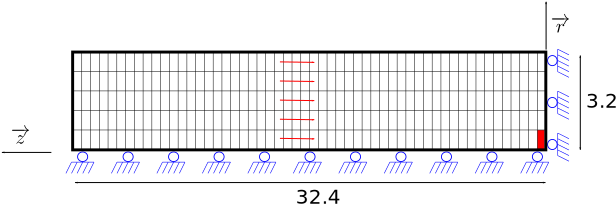
\includegraphics[width=0.75\columnwidth]{Figures/TaylorAxi}
\par\end{centering}
\caption{Numerical model for the Axisymmetric Taylor impact test\label{fig:Samples!Impact!TaylorAxi}}
\end{figure}

Figure \ref{fig:Samples!Impact!TaylorAxi-temp-contour} shows the
temperature contourplot of the deformed rod for both the \DynELA~and
Abaqus. The distributions of the temperatures are almost the same
for both models. The maximum temperature $T$ is located into the
center element of the model (the red element in Figure \ref{fig:Samples!Impact!TaylorAxi})
and the models give quite the same results as reported in Table \ref{tab:Samples!Impact!TaylorAxi-comparison}
for $\overline{\varepsilon}^{p}$, $T$ and the final dimensions of
the specimen $L_{f}$ (final length) and $D_{f}$ (final diameter
of the impacting face). 

Figure \ref{fig:Samples!Impact!TaylorAxi-comparison} shows the evolution
of the the final dimensions of the specimen $L_{f}$ (final length)
and $R_{f}$ (final radius of the impacting face), the equivalent
plastic strain $\overline{\varepsilon}^{p}$, the temperature $T$,
the von Mises stress $\overline{\sigma}$ and the timeStep $\Delta t$
for the different models for the element at the center of the impacting
face (the red element in Figure \ref{fig:Samples!Impact!TaylorAxi}). 

As reported in this figure and according to the results presented
in Table \ref{tab:Samples!Impact!TaylorAxi-comparison}, a quite good
agreement between the results is obtained.

\begin{figure}[h]
\begin{centering}
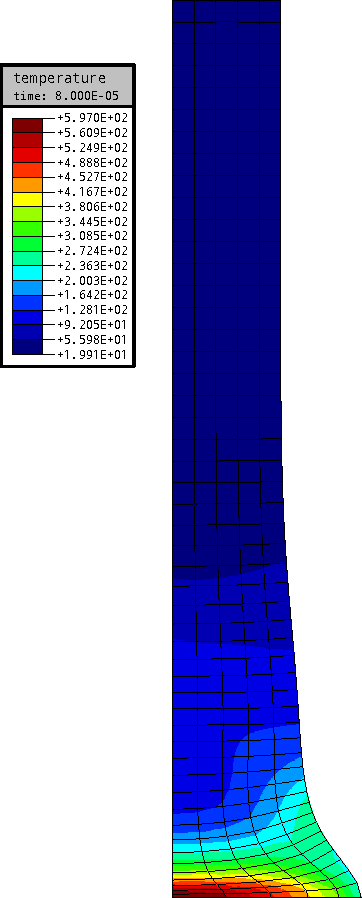
\includegraphics[height=0.5\columnwidth]{Figures/Samples/Impact/Taylor-Axi_temperatureCP}\hspace*{3cm}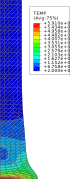
\includegraphics[height=0.5\columnwidth]{Figures/Samples/Impact/Taylor-Axi-Abaqus_Temperature}
\par\end{centering}
\caption{Temperature contourplots for Axisymmetric Taylor impact test (DynELA
left and Abaqus right)\label{fig:Samples!Impact!TaylorAxi-temp-contour}}
\end{figure}

\begin{table}[h]
\begin{center}\begin{tcolorbox}[width=.75\textwidth,myTab,tabularx={C|C|C|C|C}]
code & $L_f$ & $D_f$ & $T$ & $\overline{\varepsilon}^{p}$ \\
 & \small{($mm$)} & \small{($mm$)} & \small{($^{\circ}C$)} & \\ \hline\hline
DynELA & $26.52$ & $11.15$ & $582.34$ & $1.78$ \\ \hline
Abaqus & $26.56$ & $11.16$ & $590.96$ & $1.81$
\end{tcolorbox}\end{center}\caption{Comparison of numerical results for the Axisymmetric Taylor impact
test\label{tab:Samples!Impact!TaylorAxi-comparison}}
\end{table}

\begin{figure}[h]
\begin{centering}
\begin{tabular}{cc}
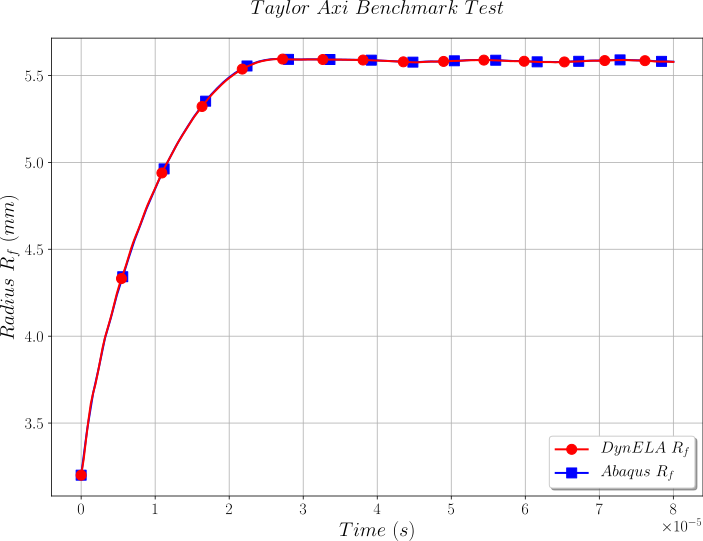
\includegraphics[width=0.45\columnwidth]{Figures/Samples/Impact/Taylor-Axi_radius} & 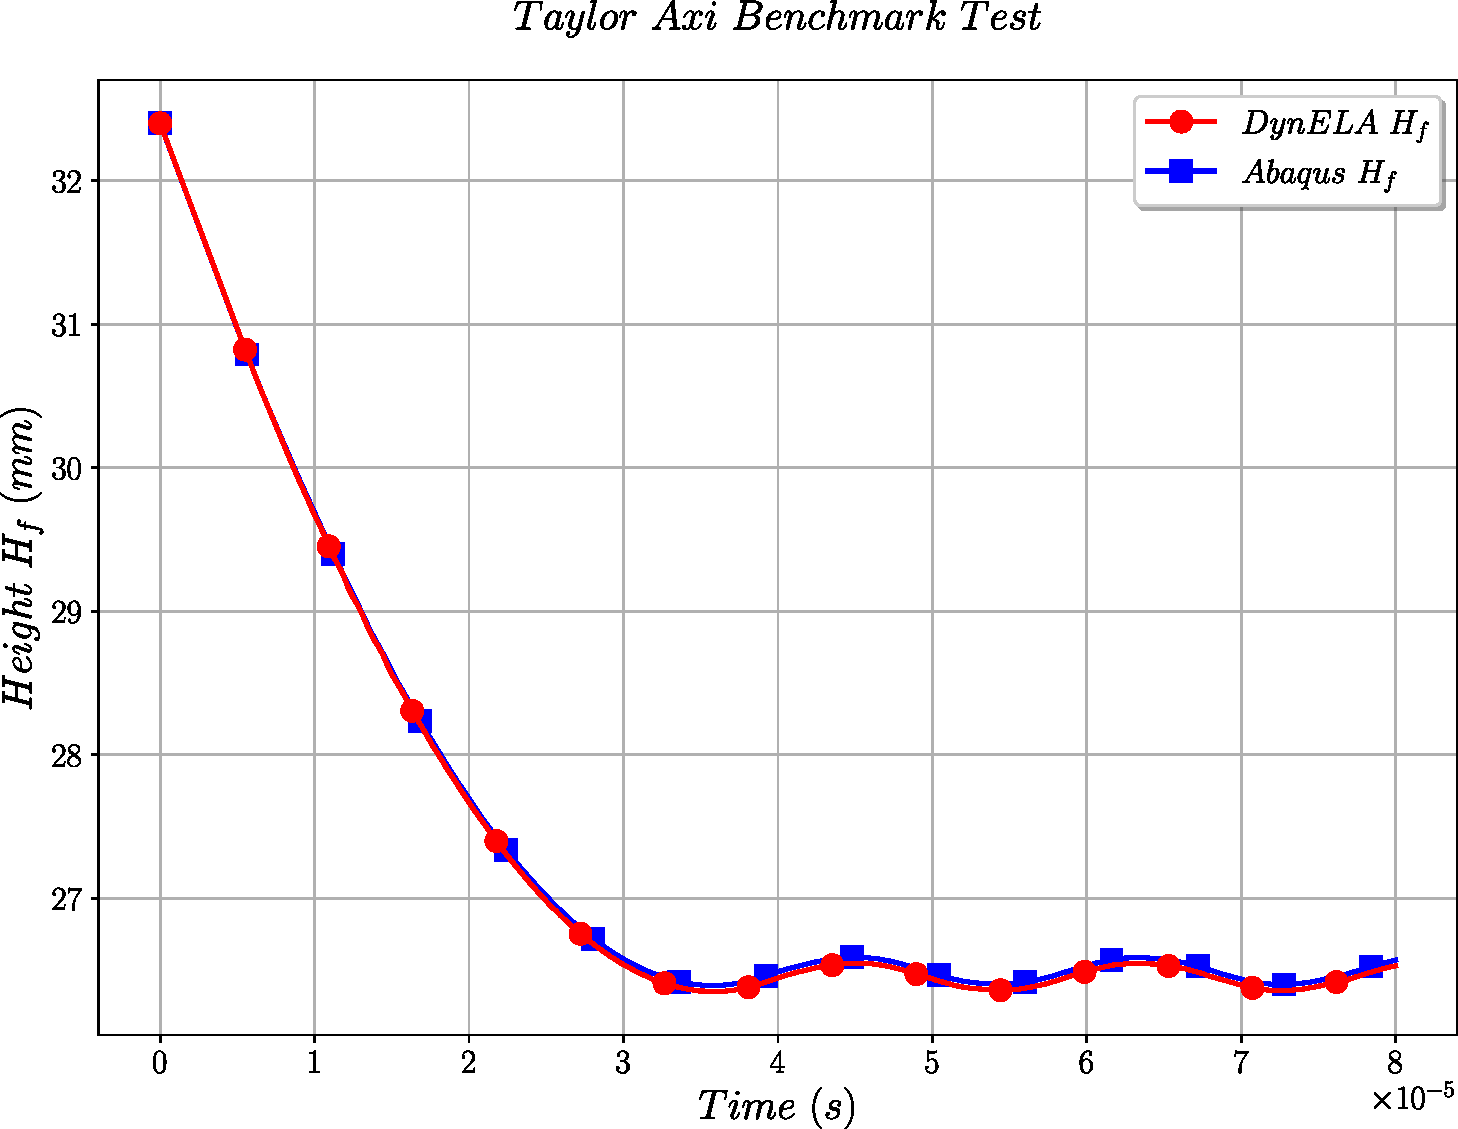
\includegraphics[width=0.45\columnwidth]{Figures/Samples/Impact/Taylor-Axi_height}\tabularnewline
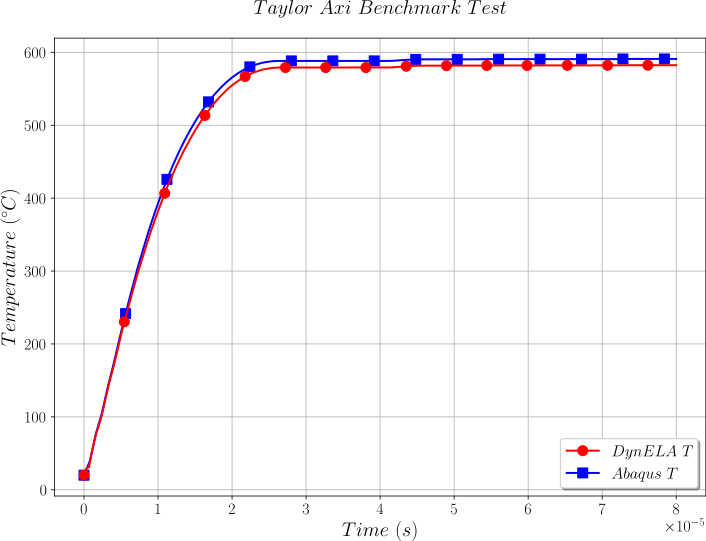
\includegraphics[width=0.45\columnwidth]{Figures/Samples/Impact/Taylor-Axi_temperature} & 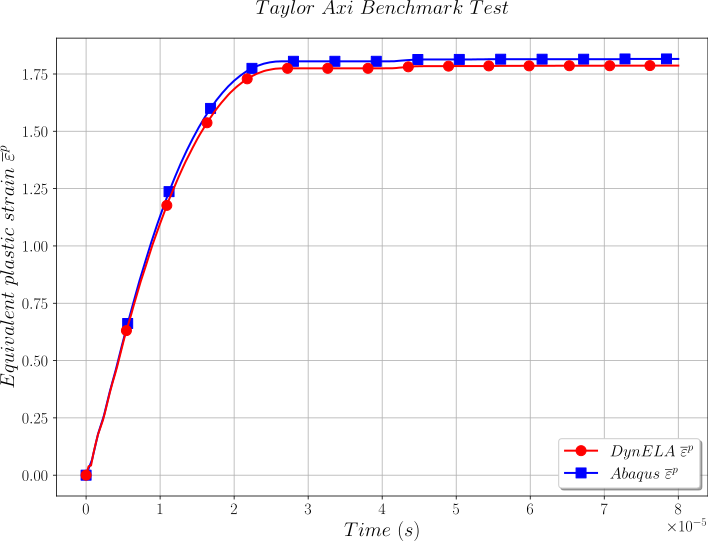
\includegraphics[width=0.45\columnwidth]{Figures/Samples/Impact/Taylor-Axi_plasticStrain}\tabularnewline
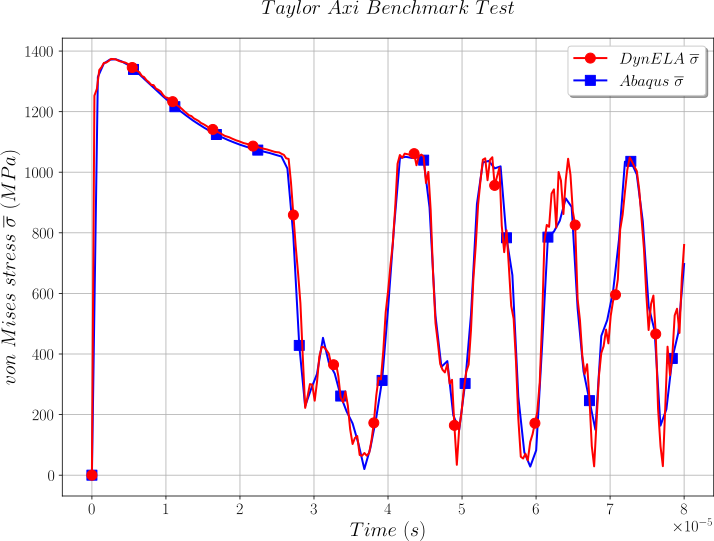
\includegraphics[width=0.45\columnwidth]{Figures/Samples/Impact/Taylor-Axi_vonMises} & 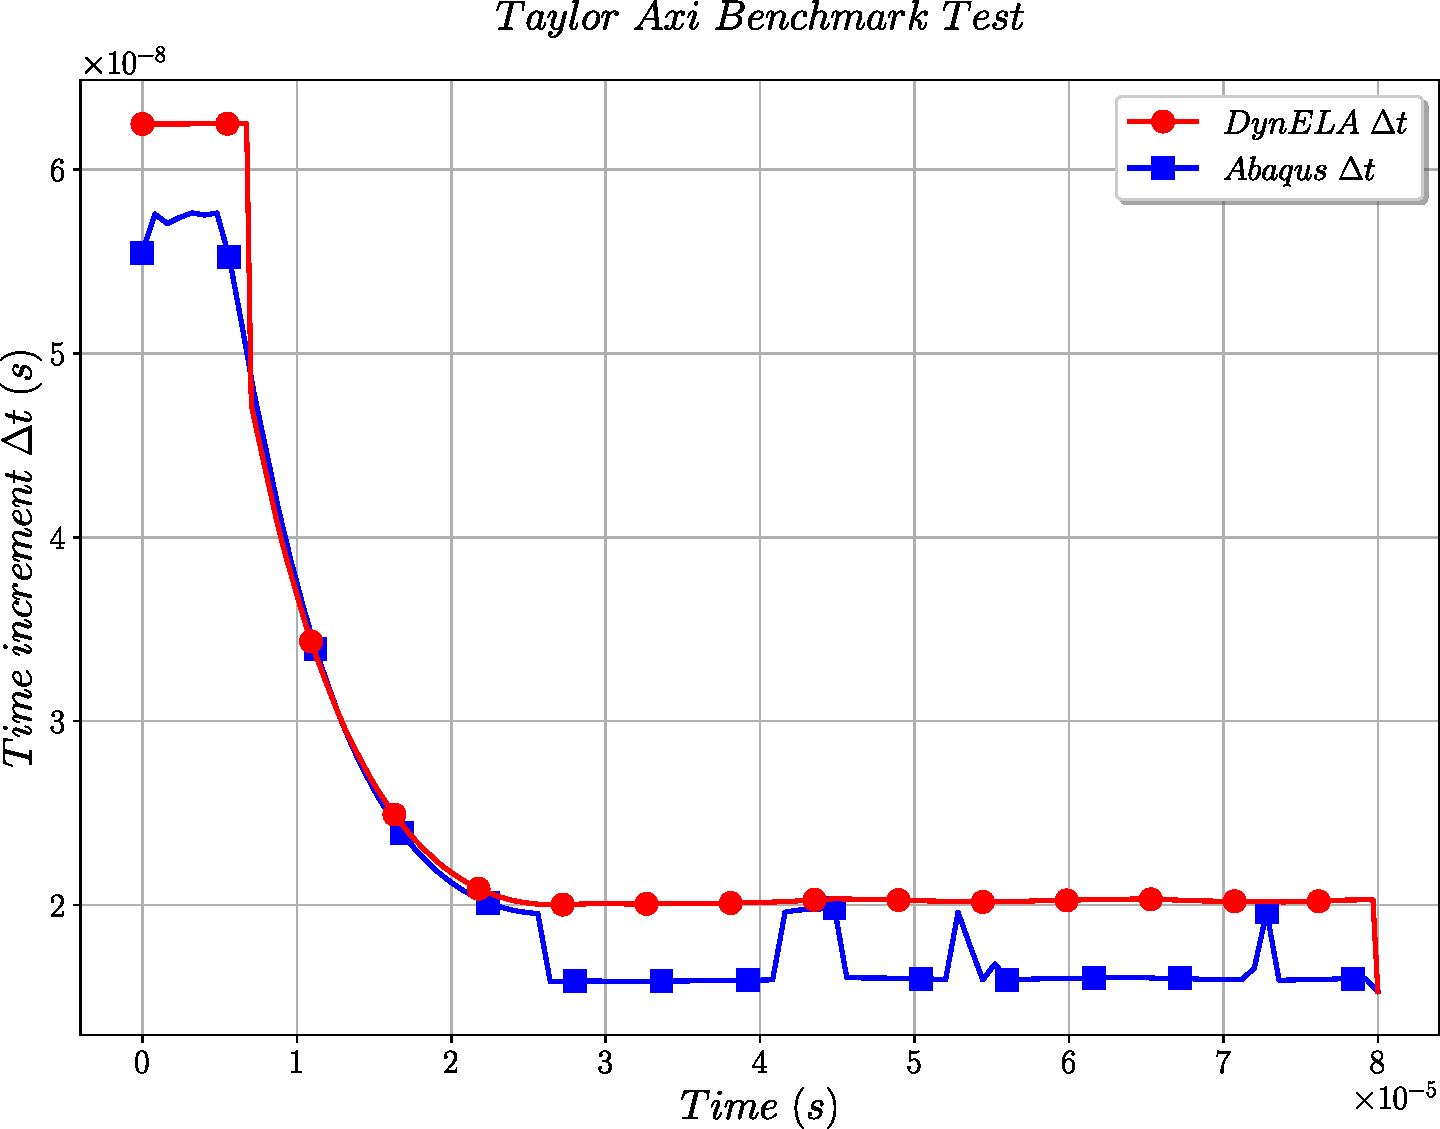
\includegraphics[width=0.45\columnwidth]{Figures/Samples/Impact/Taylor-Axi_timeStep}\tabularnewline
\end{tabular}
\par\end{centering}
\caption{Comparison of numerical and analytical results for the Axisymmetric
Taylor impact test\label{fig:Samples!Impact!TaylorAxi-comparison}}
\end{figure}


\subsection{3D Taylor impact}

The performance of the proposed code is validated under high deformation
rate with the simulation of the Taylor impact test \cite{taylor1946james}.
In the Taylor impact test, a cylindrical specimen is launched to impact
a rigid target with a prescribed initial velocity. The numerical model,
reported in Figure \ref{fig:Samples!Impact!Taylor3D} is established
as axisymmetric. The height is $32.4\,mm$ and the radius is $3.2\,mm$.
The axial displacement is restrained on the right side of the specimen
while the radial displacement is free (to figure a perfect contact
without friction of the projectile onto the target). A predefined
velocity of $V_{c}=287\,m/s$ is imposed on the specimen. The mesh
consists of $4455$ elements ($55\times81$ elements). The total simulation
time for the Taylor impact test is $t=8.0\,10^{-5}s$.

\begin{figure}[h]
\begin{centering}
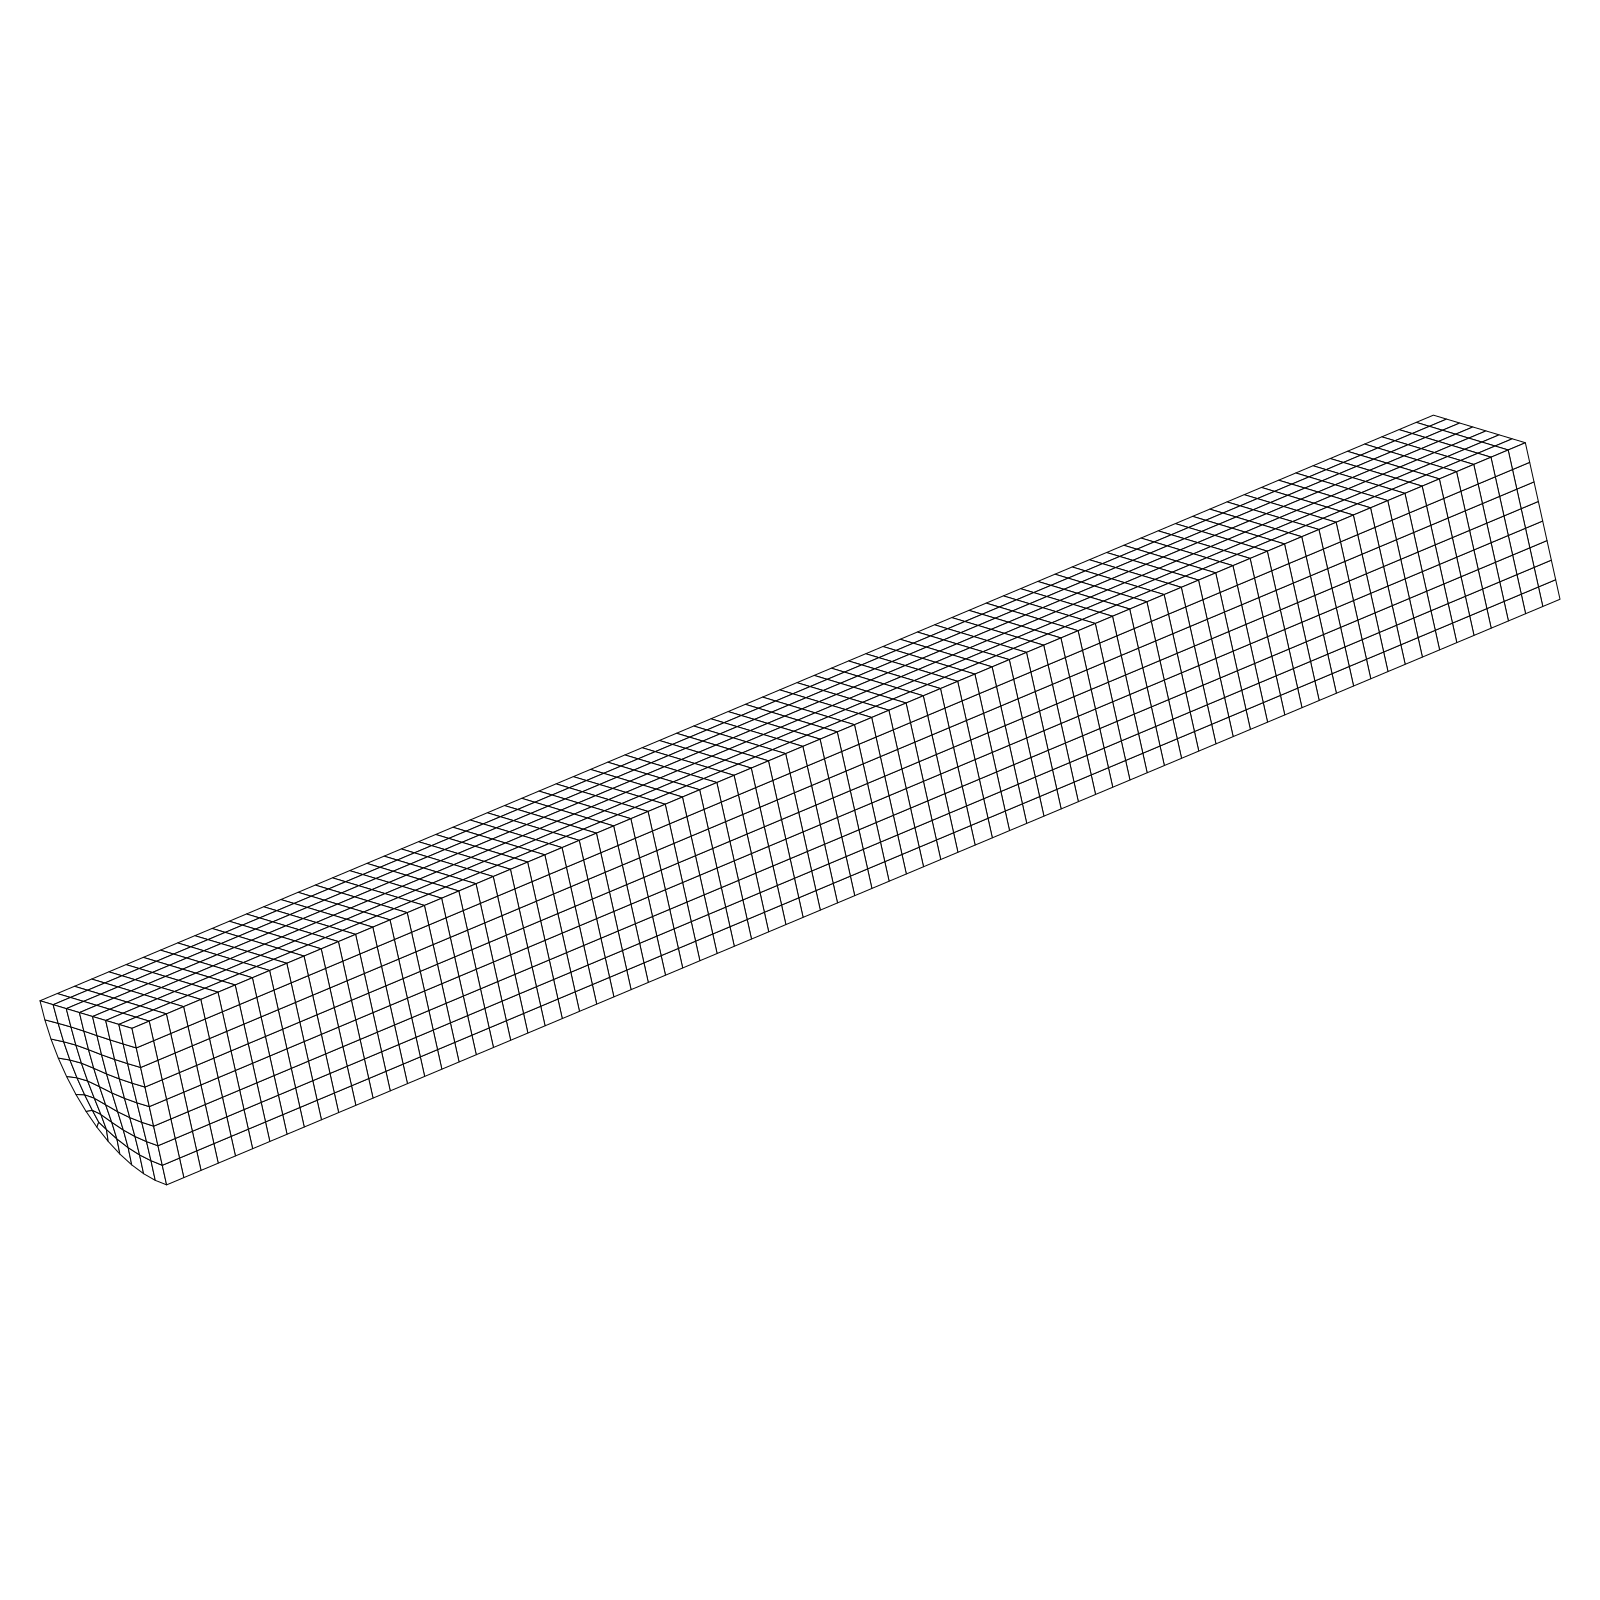
\includegraphics[width=0.5\columnwidth]{Figures/Samples/Impact/Taylor-3D_mesh}
\par\end{centering}
\caption{Numerical model for the 3D Taylor impact test\label{fig:Samples!Impact!Taylor3D}}
\end{figure}

Figure \ref{fig:Samples!Impact!Taylor3D-temp-contour} shows the temperature
contourplot of the deformed rod for both the \DynELA~and Abaqus.
The distributions of the temperatures are almost the same for both
models. The maximum temperature $T$ is located into the center element
of the model (the red element in Figure \ref{fig:Samples!Impact!Taylor3D})
and the models give quite the same results as reported in Table \ref{tab:Samples!Impact!Taylor3D-comparison}
for $\overline{\varepsilon}^{p}$, $T$ and the final dimensions of
the specimen $L_{f}$ (final length) and $D_{f}$ (final diameter
of the impacting face). 

Figure \ref{fig:Samples!Impact!Taylor3D-comparison} shows the evolution
of the the final dimensions of the specimen $L_{f}$ (final length)
and $R_{f}$ (final radius of the impacting face), the equivalent
plastic strain $\overline{\varepsilon}^{p}$, the temperature $T$,
the von Mises stress $\overline{\sigma}$ and the timeStep $\Delta t$
for the different models for the element at the center of the impacting
face (the red element in Figure \ref{fig:Samples!Impact!Taylor3D}). 

As reported in this figure and according to the results presented
in Table \ref{tab:Samples!Impact!Taylor3D-comparison}, a quite good
agreement between the results is obtained.

\begin{figure}[h]
\begin{centering}
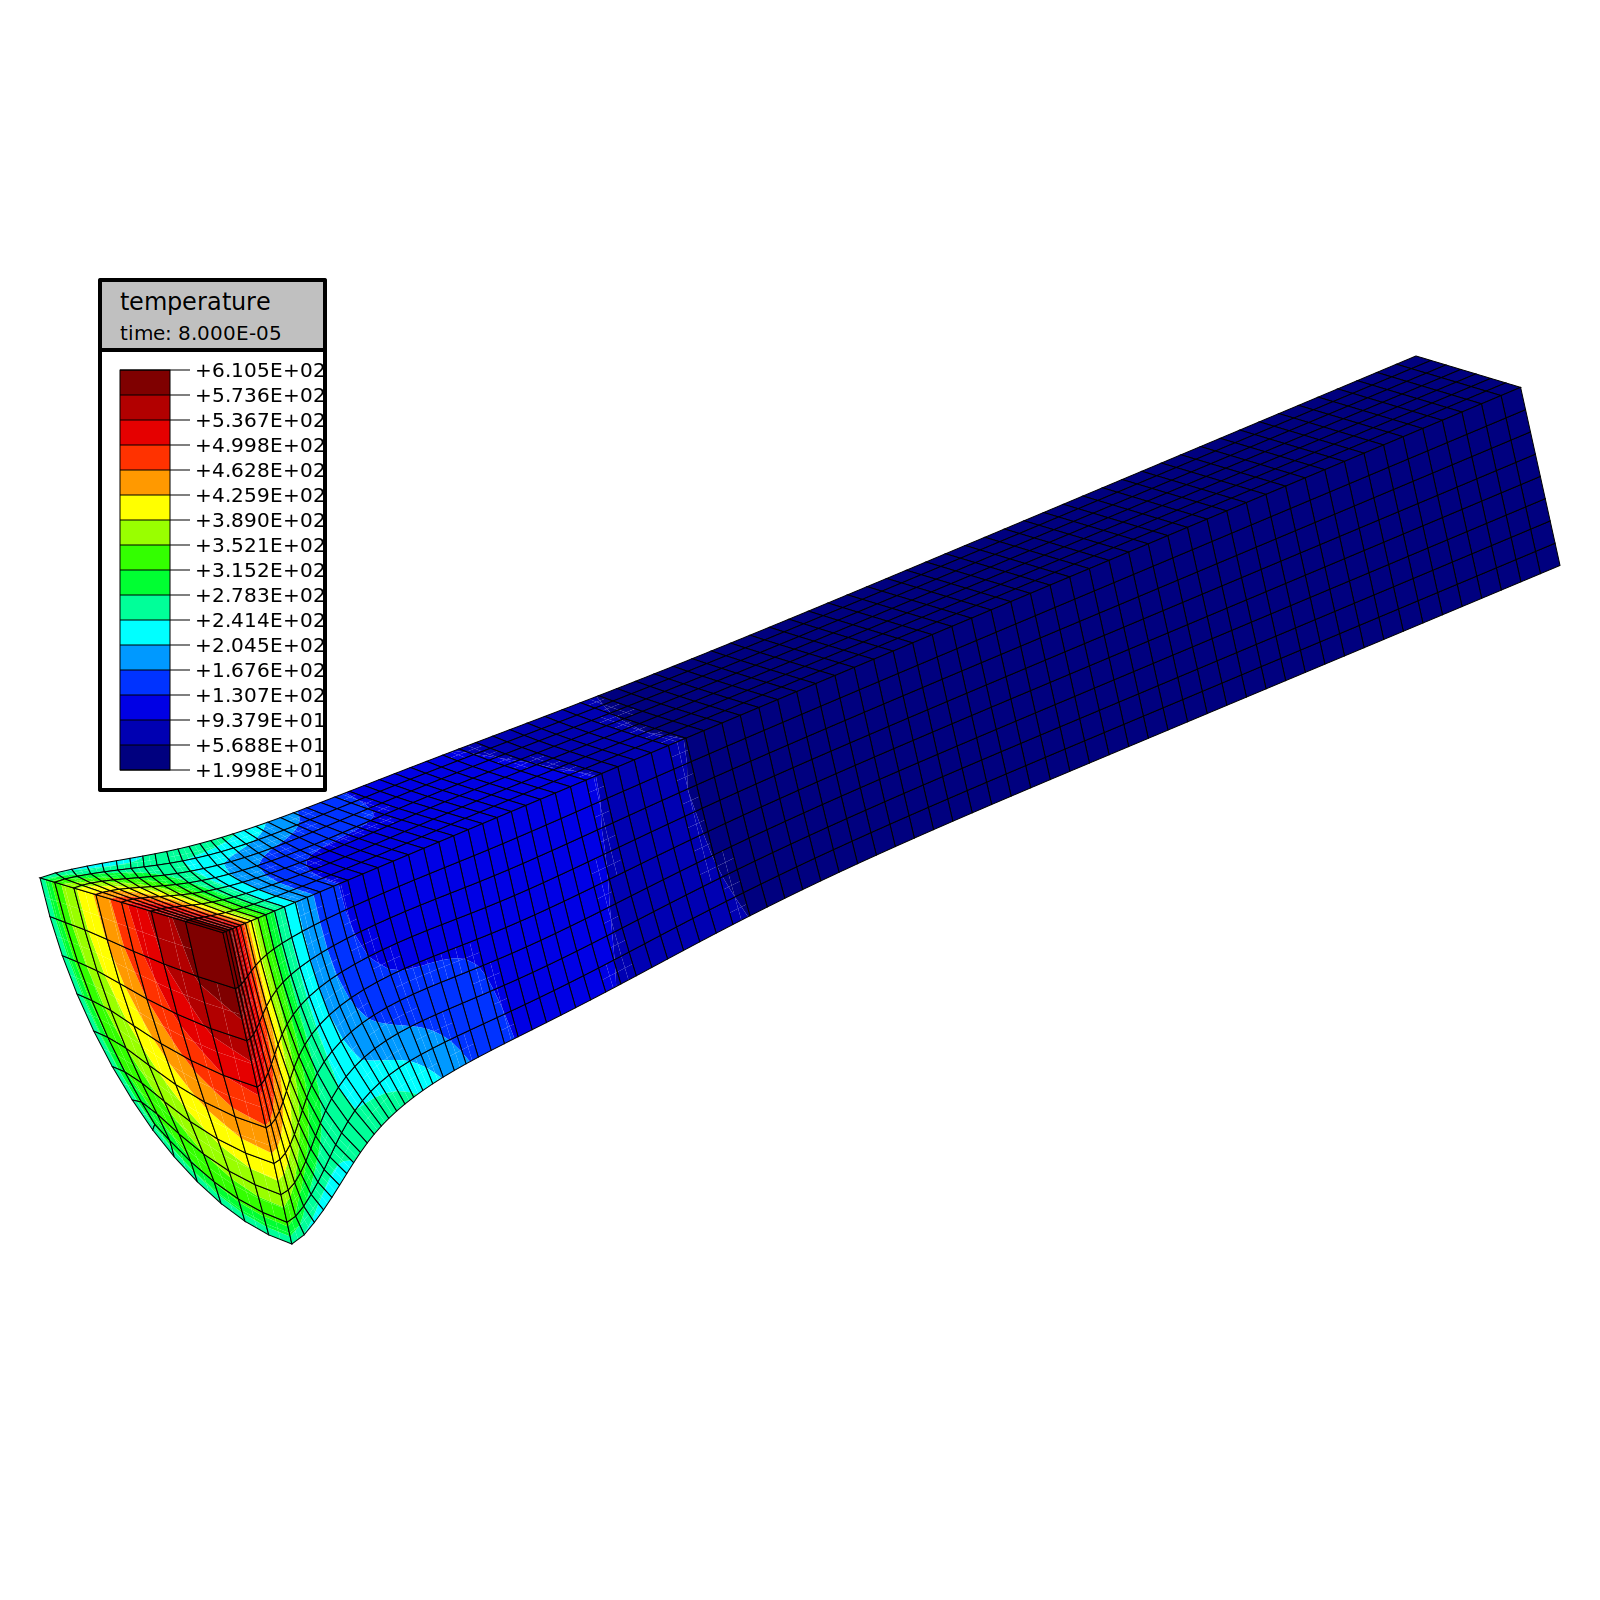
\includegraphics[width=0.8\columnwidth]{Figures/Samples/Impact/Taylor-3D_temperatureCP}
\par\end{centering}
\caption{Temperature contourplot for the 3D Taylor impact test\label{fig:Samples!Impact!Taylor3D-temp-contour}}
\end{figure}

\begin{table}[h]
\begin{center}\begin{tcolorbox}[width=.75\textwidth,myTab,tabularx={C|C|C|C|C}]
code & $L_f$ & $D_f$ & $T$ & $\overline{\varepsilon}^{p}$ \\
 & \small{($mm$)} & \small{($mm$)} & \small{($^{\circ}C$)} & \\ \hline\hline
DynELA & $26.52$ & $11.18$ & $597.10$ & $1.84$ \\ \hline
Abaqus & $26.55$ & $11.22$ & $597.01$ & $1.84$
\end{tcolorbox}\end{center}\caption{Comparison of numerical results for the 3D Taylor impact test\label{tab:Samples!Impact!Taylor3D-comparison}}
\end{table}

\begin{figure}[h]
\begin{centering}
\begin{tabular}{cc}
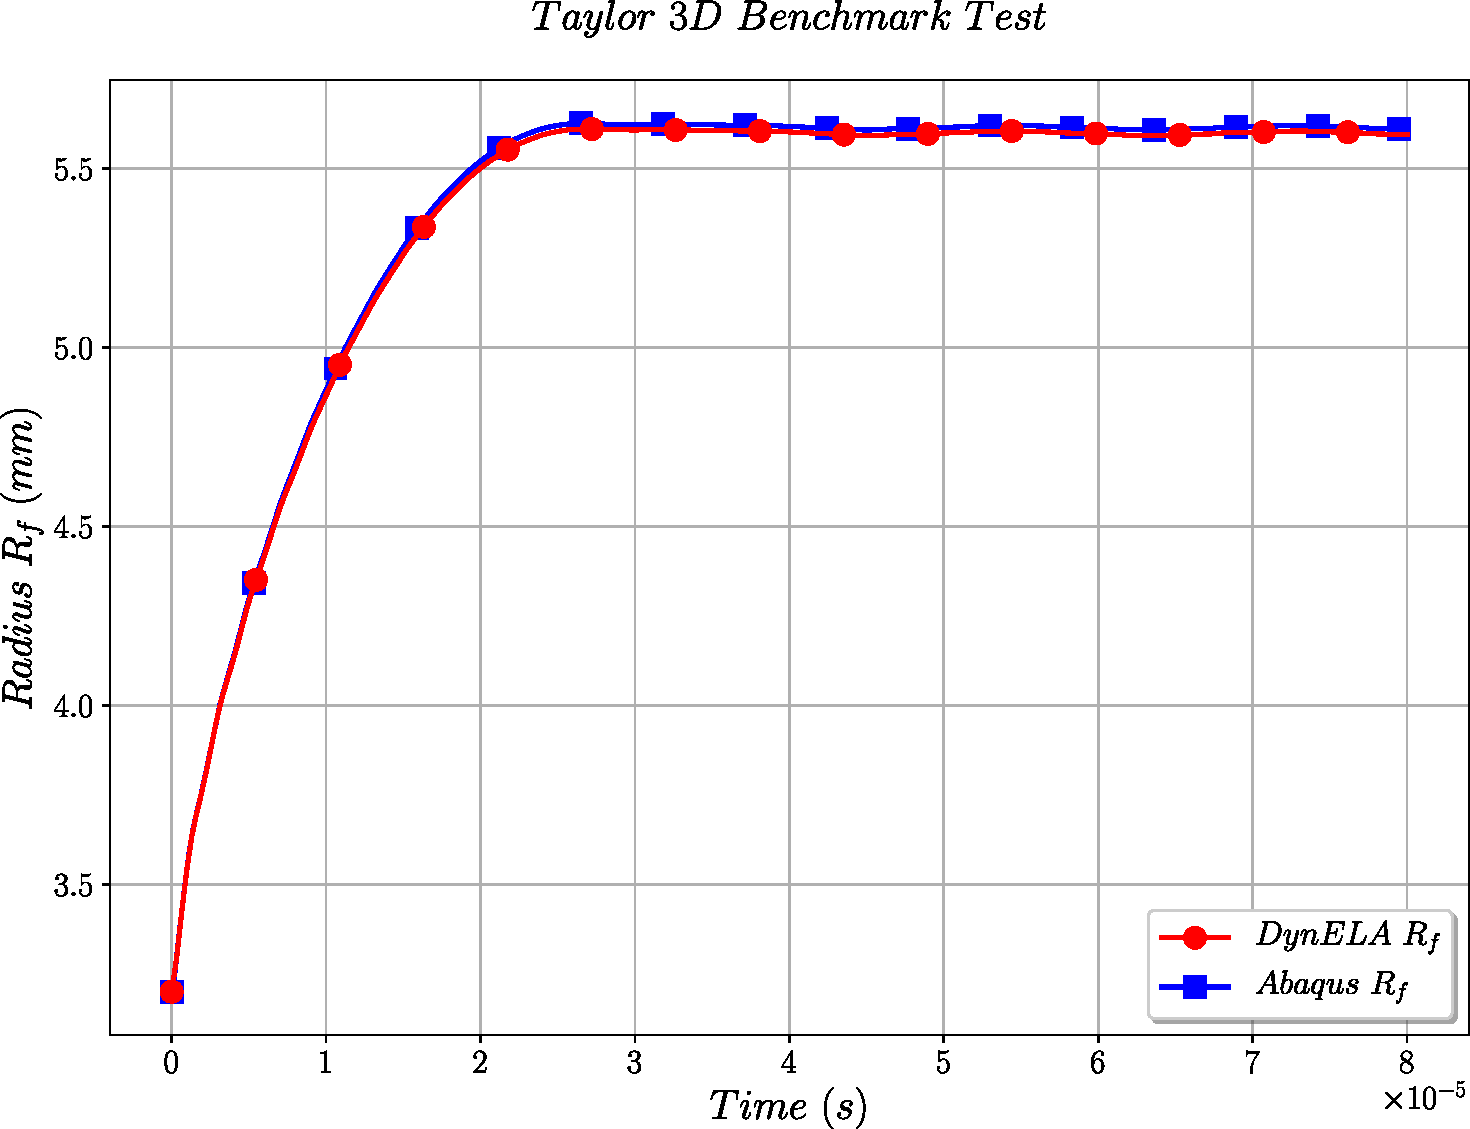
\includegraphics[width=0.45\columnwidth]{Figures/Samples/Impact/Taylor-3D_radius} & 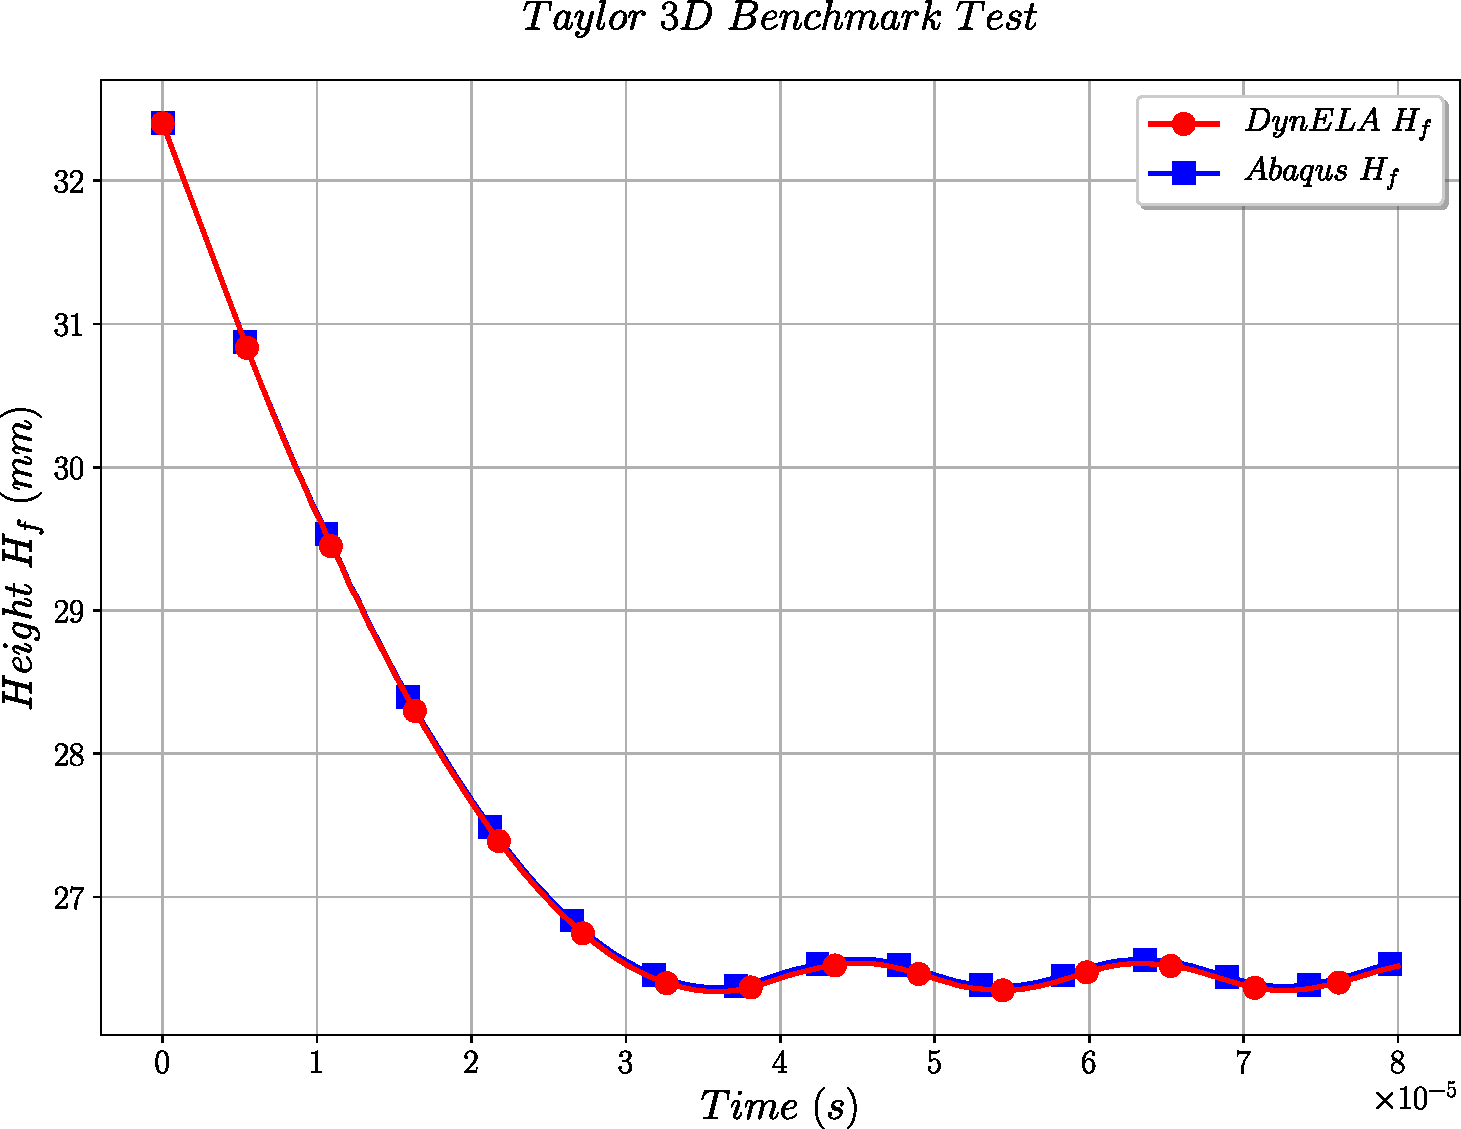
\includegraphics[width=0.45\columnwidth]{Figures/Samples/Impact/Taylor-3D_height}\tabularnewline
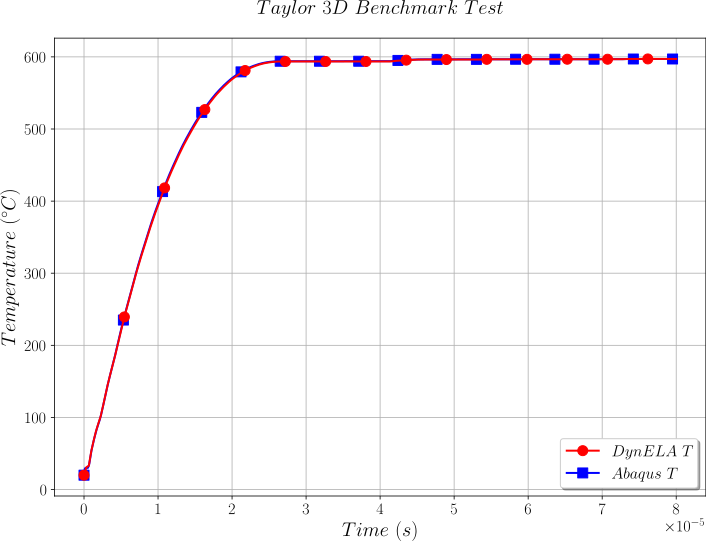
\includegraphics[width=0.45\columnwidth]{Figures/Samples/Impact/Taylor-3D_temperature} & 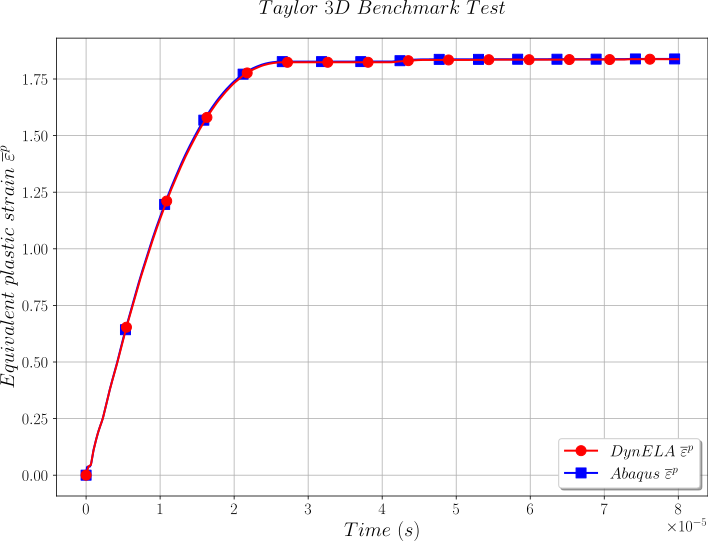
\includegraphics[width=0.45\columnwidth]{Figures/Samples/Impact/Taylor-3D_plasticStrain}\tabularnewline
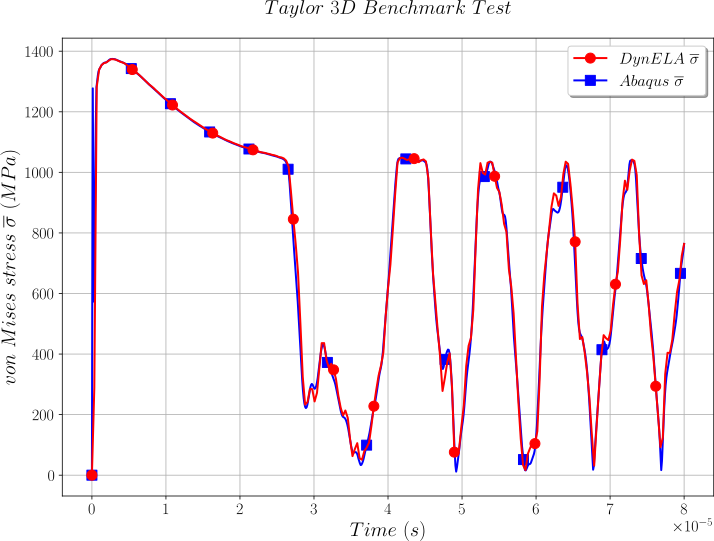
\includegraphics[width=0.45\columnwidth]{Figures/Samples/Impact/Taylor-3D_vonMises} & 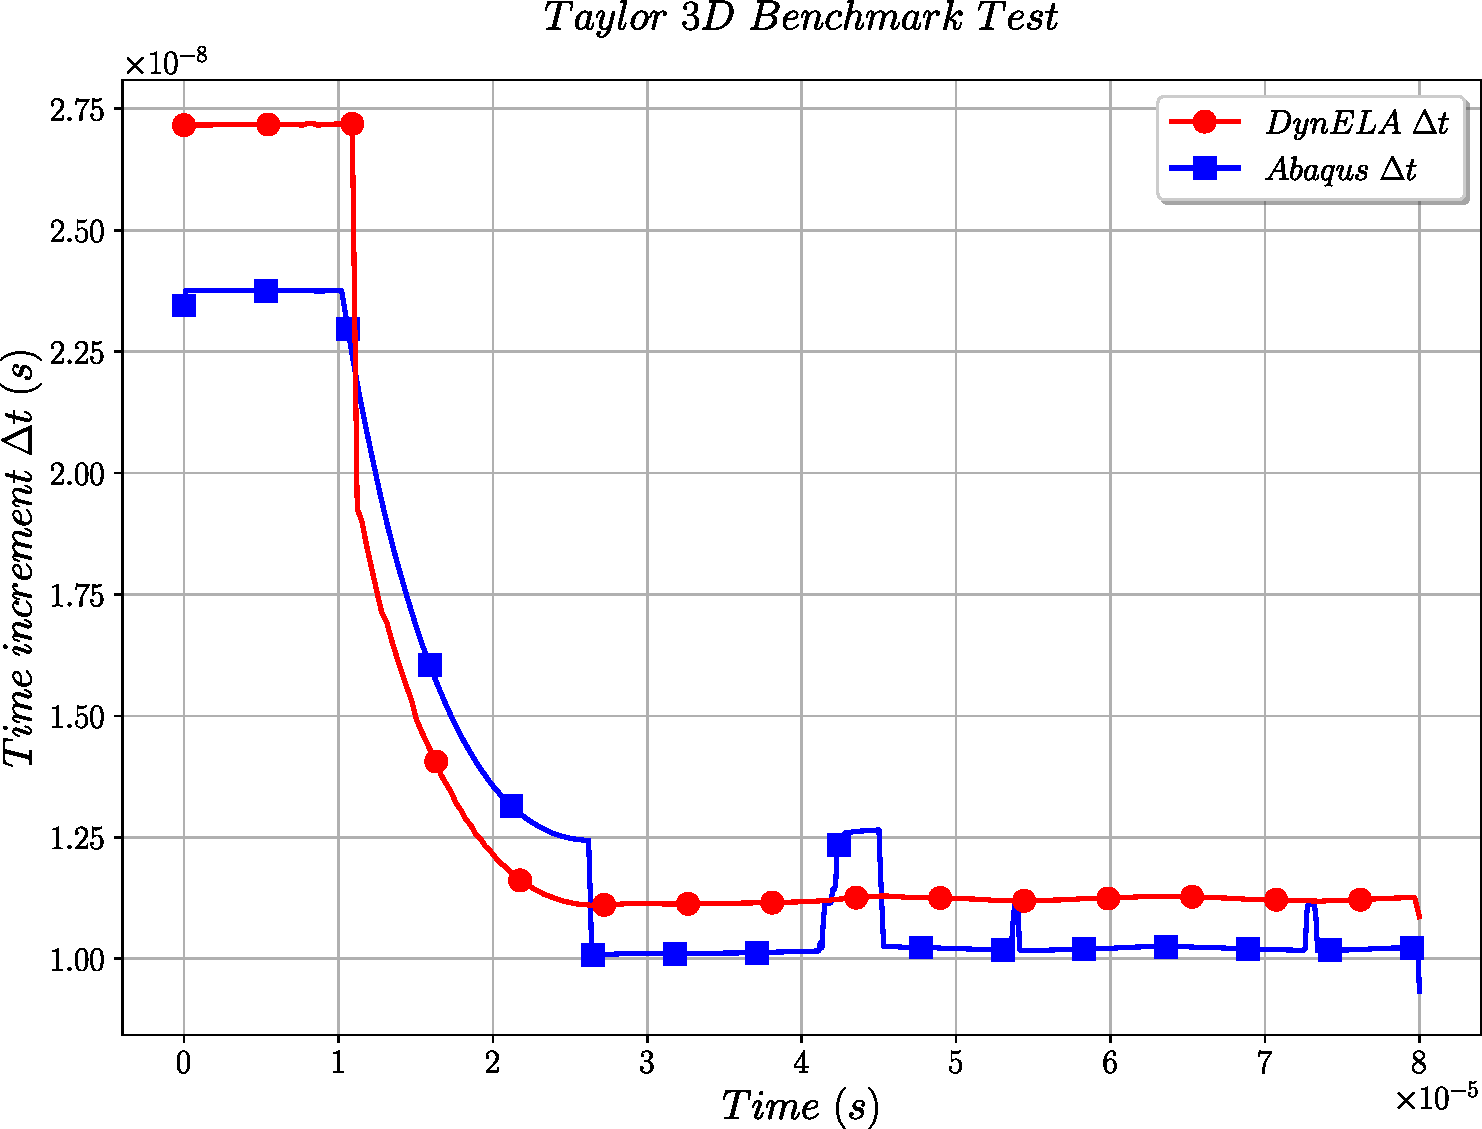
\includegraphics[width=0.45\columnwidth]{Figures/Samples/Impact/Taylor-3D_timeStep}\tabularnewline
\end{tabular}
\par\end{centering}
\caption{Comparison of numerical and analytical results for the 3D Taylor impact
test\label{fig:Samples!Impact!Taylor3D-comparison}}
\end{figure}

